\section{Preliminaries}
\label{preliminary}

\begin{figure}[ht]
    \centering
    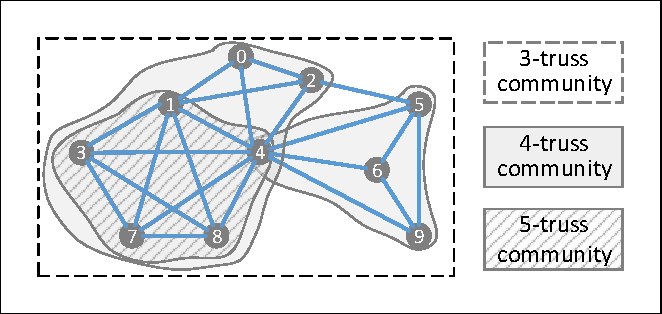
\includegraphics[width=0.7\linewidth, trim={0.1cm 0.1cm, 0.1cm, 0.1cm}, clip]{./figures/k-truss.pdf}
    \caption{An example graph with four k-truss communities}
    \label{fig:example}
\end{figure}

In our problem, we consider an undirected, unweighted graph $G = (V,E)$. An example graph is shown in \autoref{fig:example}.
%The number of vertices is denoted as $n = |V|$ and number of edges is denoted as $m = |E|$. 
%We use $w_u$ and $w_e$ to denote the weight of a vertex $u$ and an edge $e$. 
We define the set of neighbors of a vertex $v$ in $G$ as $N_v = {u \in V :(v, u) \in E}$, and the degree of $v$ as $d_v = |N_v|$. We define a triangle $\triangle_{uvw}$ as a cycle of length $3$ with distinct vertices $u, v, w \in V$. 
Then we define several key concepts as follows.

\begin{Def}[Edge support]
The support of an edge $e_{u,v} \in E$ is defined as $s_{e,G} = |{\triangle_{uvw} : w \in V}|$. 
We denote it as $s_e$ when the context is clear.
\label{def:edge_support}
\end{Def}

For example, in \autoref{fig:example}, the edge support for $(0,2)$ is $2$, as it is contained in triangle $(0,2,1)$ and triangle $(0,2,4)$.

\begin{Def}[Trussness] 
The trussness of a subgraph $G^{\prime} \in G$ is the minimum support of edges in $G^{\prime}$ plus $2$, denoted by $\tau_{G^{\prime}} = min\{(s_{e,G^{\prime}} + 2): e \in E_{G^{\prime}}\} $.  We then define edge trussness as: $\tau_{e} = max_{G^{\prime} \in G}\{\tau_{G^{\prime}}: e \in E_{G^{\prime}}\}$.
\label{def:trussness}
\end{Def}

For example, in \autoref{fig:example}, subgraph $(1,3,7,8,4)$ has trussness of $5$ as all edges in it have support at least $5-2=3$. The trussness for edge $(1,4)$ is $5$, as subgraph $(1,3,7,8,4)$ has trussness of $5$.

\begin{Def}[K-truss]
Given a graph $G$ and $k \ge 2$, $G^{\prime} \subseteq G$ is a k-truss if $\forall e \in E_{G^{\prime}}, s_{e,G^{\prime}} \ge (k - 2)$. 
$G^{\prime}$ is a maximal k-truss subgraph if it is not a subgraph of another k-truss subgraph with the same trussness $k$ in $G$.
\label{def:k-truss}
\end{Def}

%\begin{Def}[Maximal k-truss subgraph]
%$H$ is a maximal k-truss subgraph if it is not a subgraph of another k-truss subgraph with same trussness $k$ in $G$.
%\label{def:maximal_k-truss}
%\end{Def}

Because the K-truss definition does not define the connectivity of the subgraph, we have the following definitions for triangle connectivity.

\begin{Def}[Triangle adjacency]
${\triangle}_{1}$, ${\triangle}_{2}$ are adjacent if they share a common edge, i.e., ${\triangle}_{1} \cap {\triangle}_{2} \neq \emptyset$. 
\label{def:triangle_adjacency}
\end{Def}

\begin{Def}[Triangle connectivity] 
${\triangle}_{1}$, ${\triangle}_{2}$ are triangle connected if they can reach each other through a series of adjacent triangles, \ie for $1 \le i < n, {\triangle}_{i} \cap {\triangle}_{i-1} \neq \emptyset$. Two edges $e_1$, $e_2$ are triangle connected if $\exists e_{1} \in {\triangle}_{1}$, $e_{2} \in {\triangle}_{2}$, ${\triangle}_{1}$ and ${\triangle}_{2}$ are identical or triangle connected.
\label{def:triangle_connectivity}
\end{Def}

For example, in \autoref{fig:example}, $(1,4)$ is triangle connected to $(5,6)$ through a series of adjacent triangles $(1,2,4)$, $(2,4,5)$ and $(4,5,6)$.

%\begin{Def}[Triangle connected graph]
%Two edge $e_{1}, e_{2}$ are triangle connected in a subgraph $H$ if there are two triangle ${\triangle}_{1}, {\triangle}_{2}$ in $H$ and $e_{1} \in {\triangle}_{1}, e_{2} \in {\triangle}_{2}$, either ${\triangle}_{1} = {\triangle}_{2}$, or ${\triangle}_{1}$ is triangle connected with ${\triangle}_{2}$ in $H$.
%A graph $G$ is triangle connected if all pairs of edges in $G$ are triangle connected.
%\label{def:triangle_connected_graph}
%\end{Def}

Finally, we define k-truss community based on the definition of k-truss subgraph and triangle connectivity as follows.

\begin{Def}[K-truss community] 
A k-truss community is a maximal k-truss subgraph and all its edges are triangle connected.
\label{def:k-truss_community}
\end{Def}

fig:example shows several examples of k-truss communities. The whole example graph is a $3$-truss community as every edge has the support of at least 1 and all edges are triangle connected with each other. Note that there are two separate $4$-truss communities in \autoref{fig:example}. Because the edge support of edge $(2,5)$ is only $1$, it cannot belong to a $4$-truss. After excluding edge $(2,5)$, edges in the two $4$-trusses are no longer triangle connected.
%The problem studied in this paper is to build index structures to answer K-truss community related queries.
%defined as follows. Given a graph $G(V,E)$, a set of query vertices $Q \in V$, find all truss communities containing $Q$ with maximum $k$, a specific $k$ or any possible $k$. 